\documentclass[10pt]{exam}

\usepackage{amssymb, amsmath, amsthm, mathrsfs, multicol, graphicx}
\usepackage{tikz}

 \def\d{\displaystyle}
\def\?{\reflectbox{?}}
\def\b#1{\mathbf{#1}}
\def\f#1{\mathfrak #1}
\def\c#1{\mathcal #1}
\def\s#1{\mathscr #1}
\def\r#1{\mathrm{#1}}
\def\N{\mathbb N}
\def\Z{\mathbb Z}
\def\Q{\mathbb Q}
\def\R{\mathbb R}
\def\C{\mathbb C}
\def\F{\mathbb F}
\def\A{\mathbb A}
\def\X{\mathbb X}
\def\E{\mathbb E}
\def\O{\mathbb O}
\def\U{\mathcal U}
\def\pow{\mathcal P}
\def\inv{^{-1}}
\def\nrml{\triangleleft}
\def\st{:}
\def\~{\widetilde}
\def\rem{\mathcal R}
\def\sigalg{$\sigma$-algebra }
\def\Gal{\mbox{Gal}}
\def\iff{\leftrightarrow}
\def\Iff{\Leftrightarrow}
\def\land{\wedge}
\def\And{\bigwedge}
\def\AAnd{\d\bigwedge\mkern-18mu\bigwedge}
\def\Vee{\bigvee}
\def\VVee{\d\Vee\mkern-18mu\Vee}
\def\imp{\rightarrow}
\def\Imp{\Rightarrow}
\def\Fi{\Leftarrow}

%\def\={\equiv}
\def\var{\mbox{var}}
\def\mod{\mbox{Mod}}
\def\Th{\mbox{Th}}
\def\sat{\mbox{Sat}}
\def\con{\mbox{Con}}
\def\bmodels{=\joinrel\mathrel|}
\def\iffmodels{\bmodels\models}
\def\dbland{\bigwedge \!\!\bigwedge}
\def\dom{\mbox{dom}}
\def\rng{\mbox{range}}
\DeclareMathOperator{\wgt}{wgt}


\def\bar{\overline}


\newcommand{\vtx}[2]{node[fill,circle,inner sep=0pt, minimum size=4pt,label=#1:#2]{}}
\newcommand{\va}[1]{\vtx{above}{#1}}
\newcommand{\vb}[1]{\vtx{below}{#1}}
\newcommand{\vr}[1]{\vtx{right}{#1}}
\newcommand{\vl}[1]{\vtx{left}{#1}}
\renewcommand{\v}{\vtx{above}{}}

\def\circleA{(-.5,0) circle (1)}
\def\circleAlabel{(-1.5,.6) node[above]{$A$}}
\def\circleB{(.5,0) circle (1)}
\def\circleBlabel{(1.5,.6) node[above]{$B$}}
\def\circleC{(0,-1) circle (1)}
\def\circleClabel{(.5,-2) node[right]{$C$}}
\def\twosetbox{(-2,-1.4) rectangle (2,1.4)}
\def\threesetbox{(-2.5,-2.4) rectangle (2.5,1.4)}
\newcommand{\twoline}[2]{\begin{pmatrix}#1 \\ #2 \end{pmatrix}}


\def\circleA{(-.5,0) circle (1)}
\def\circleAlabel{(-1.5,.6) node[above]{$A$}}
\def\circleB{(.5,0) circle (1)}
\def\circleBlabel{(1.5,.6) node[above]{$B$}}
\def\circleC{(0,-1) circle (1)}
\def\circleClabel{(.5,-2) node[right]{$C$}}
\def\twosetbox{(-2,-1.5) rectangle (2,1.5)}
\def\threesetbox{(-2,-2.5) rectangle (2,1.5)}

%\pointname{pts}
\pointsinmargin
\marginpointname{pts}
\bonuspointname{pts}
\marginbonuspointname{pts}
\addpoints
\pagestyle{head}
%\printanswers

\firstpageheader{Math 228}{\bf Homework 7}{Due: Wednesday, October 18}


\begin{document}
\noindent \textbf{Instructions}: Same rules as usual -- turn in your work on separate sheets of paper.  You must justify all your answers for full credit.  Do not consult the Internet.

\begin{questions}



\question[6] On the way to the market, you exchange your cow for some magic dark chocolate espresso beans.  These beans have the property that every night at midnight, each bean splits into two, effectively doubling your collection.  You decide to take advantage of this and each morning (around 8am) you eat 5 beans.
\begin{parts}
\part Explain why it is true that \emph{if} at noon on day $n$ you have a number of beans ending in a 5, then at noon on day $n+1$ you will still have a number of beans ending in a 5.

\begin{solution}
If we have a number of beans ending in a 5 and we double it, we will get a number of beans ending in a 0 (since $5\cdot 2 = 10$).  Then if we subtract 5, we will once again get a number of beans ending in a 5.  Thus if on any day we have a number ending in a 5, the next day will also have a number ending in a 5.

\end{solution}

\part Why is the previous fact not enough to conclude that you will always have a number of beans ending in a 5? What additional fact would you need?
\begin{solution}
If you don't \emph{start} with a number of beans ending in a 5 (on day 1), the above reasoning is still correct but not helpful.  For example, if you start with a number ending in a 3, the next day you will have a number ending in a 1.
\end{solution}

\part Assuming you have the additional fact in part (b), and have successfully proved the fact in part (a), how do you know that you will always have a number of beans ending in a 5?  Illustrate what is going on by carefully explaining how the two facts above prove that you will have a number of beans ending in a 5 on \textbf{day 4} specifically.  In other words, explain why induction works in this context.
\begin{solution}
Part (b) is the base case and part (a) is the inductive case.  If on day 1 we have a number ending in a 5 (by part (b)), then on day 2 we will also have a number ending in a 5 (by part (a)).  Then by part (a) again, we will have a number ending in a 5 on day 3.  By part (a) again, this means we will have a number ending in a 5 on day 4.

The proof by induction would say that on \emph{every} day we will have a number ending in a 5, and this works because we can start with the base case, then use the inductive case over and over until we get up to our desired $n$.
\end{solution}
\end{parts}


\uplevel{{\bf Special Induction Instructions}: For the rest of the homework problems, you should first give a rough sketch of the argument (i.e., say {\em why} induction will work in this case) and then also give a formal proof by induction (starting with, ``For each $n$, let $P(n)$ be the statement\ldots'').}

\question[8] Find the largest number of points which a football team cannot get exactly using just 3-point field goals and 7-point touchdowns (ignore the possibilities of safeties, missed extra points, and two point conversions).  Prove your answer is correct by mathematical induction.

\begin{solution}
  First note that it is impossible to make 11 points -- if only field goals are made, the points must be a multiple of 3, if 1 touchdown is made, the possible point totals are 7, 10, 13, \ldots and two touchdowns are already too much.

  We will prove that 11 is the largest number of points which cannot be made.  In other words, any number of points greater than or equal to 12 can be made.

  \begin{proof}
    Let $P(n)$ be the statement ``it is possible to make $n$ points using touchdowns and field goals.''  We will prove $P(n)$ is true for all $n \ge 12$.

    First the base case: You can make 12 points with 4 field goals, so $P(12)$ is true.

    Now the inductive case: Assume $P(k)$ is true for some fixed $k \ge 12$.  That is, it is possible to make $k$ points.  Since $k \ge 12$, we must have made the $k$ points using either at least 2 field goals or at least 2 touchdowns, or both (because if we used just one of each we would have only 10 points).  Now if the $k$ points were accomplished with 2 (or more) field goals, then replace 2 field goals with 1 touchdown.  This increases to point total by 1, giving $k + 1$ points.  On the other hand, if the $k$ points were accomplished with $2$ (or more) touchdowns, replace 2 touchdowns with 5 field goals, again increasing the point total by 1, giving $k+1$ points.  Using one of these two substitutions, we can make $k+1$ points, so $P(k+1)$ is true, establishing the inductive case.

    Therefore by the principle of mathematical induction, $P(n)$ is true for all $n \ge 12$.
  \end{proof}
\end{solution}


\question[8] Prove, by mathematical induction, that $F_0 + F_1 + F_2 + \cdots + F_{n} = F_{n+2} - 1$, where $F_n$ is the $n$th Fibonacci number ($F_0 = 0$, $F_1 = 1$ and $F_n = F_{n-1} + F_{n-2}$).
\begin{solution}
This is saying that if we add up the first $n$ Fibonacci numbers, we will get another Fibonacci number (specifically, the $(n+2)$th one).  Induction is a good idea here because it will be easy to just add one more Fibonacci number to the sum we already have.  If we already have $F_{k+2}$ and we add $F_{k+1}$ we can use the recurrence relation to simplify this, becoming $F_{k+3}$.

  \begin{proof}
    Let $P(n)$ be the statement $F_0 + F_1 + F_2 + \cdots + F_n = F_{n+2} - 1$.  We will prove that $P(n)$ is true for all $n \ge 0$.

    Base case: $P(0)$ states that $F_0 = F_2 - 1$, which is true because $F_0 = 0$ and $F_2 = 1$.

    Inductive case:  Assume $P(k)$ is true for an arbitrary fixed $k \ge 0$.  That is, \[F_0 + F_1 + F_2 + \cdots + F_k = F_{k+2} - 1\]
    We must prove that $P(k+1)$ is true as well (i.e. that $F_0 + F_1 + \cdots +F_{k+1} = F_{k+3} - 1$).  Start with the left hand side:
    \begin{align*}
      F_0 + F_1 + F_2 + \cdots + F_k + F_{k+1} & = F_{k+2} - 1 + F_{k+1} & \mbox{ by the inductive hypothesis}\\
      & = F_{k+3} - 1 & \mbox{ by the definition of the Fibonacci numbers}
    \end{align*}
    Thus $P(k+1)$ is true.

    Therefore by the principle of mathematical induction, $P(n)$ is true for all $n \ge 0$.
  \end{proof}

\end{solution}

\question[8] Prove that the sum of the interior angles of a convex $n$-gon is $(n-2)\cdot 180^\circ$.  (A convex $n$-gon is a polygon with $n$ sides for which each interior angle is less than $180^\circ$.)  Hint: start with $(k+1)$-gon and divide it up into a $k$-gon and a triangle.

\begin{solution}
Every $n$-gon (for $n \ge 4$) can be divided into a triangle and a $(n-1)$-gon by drawing a line between two vertices one apart.  The sum of the interior angles of the $n$-gon will then be the sum of the angles in the triangle and the angles in the $(n-1)$-gon.  This shows how we can go from one case to the next.  Since we are adding a triangle, we are adding $180^\circ$ to the sum, which is what incrementing $n$ in $(n-2)\cdot 180^\circ$ does.

\begin{proof}
Let $P(n)$ be the statement, ``the sum of the interior angles of a convex $n$-gon is $(n-2)\cdot 180^\circ$.''  We will prove $P(n)$ is true for all $n \ge 3$.

Base case: When $n=3$, we have a triangle, and we know the sum of the interior angles of a triangle is $180^\circ = (3-2)\cdot 180^\circ$.  Thus $P(3)$ is true.

Inductive case: Assume $P(k)$ is true for some arbitrary $k \ge 3$.  That is, the sum of the angles of any convex $k$-gon is $(k-2)\cdot 180^\circ$.  Now consider an arbitrary convex $(k+1)$-gon.  Draw an edge between two vertices one apart (for example, between the first and third vertices counting clockwise).  Since we have at least 4 vertices, this is a new edge, and divides the $k+1$-sided polygon into a convex $k$-gon and a triangle.  The sum of the angles of the $(k+1)$-gon will be exactly the sum of the angles in the $k$-gon plus the sum of the angles of the triangle.  But the $k$-gon has sum of angles $(k-2)\cdot 180^\circ$ (by the inductive hypothesis) and the triangle has sum of angles $180^\circ$, so together the sum of the interior angles of the $(k+1)$-gon is
\[(k-2)\cdot 180^\circ + 180^\circ = ((k+1)-2)\cdot 180^\circ\]
Since we can do this for \emph{any} convex $(k+1)$-gon, we see that $P(k+1)$ is true.

Therefore, by the principle of mathematical induction, $P(n)$ is true for all $n\ge 3$.

\end{proof}

\end{solution}



\bonusquestion[5] Bonus: Given a square, you can cut the square into smaller squares by cutting along lines parallel to the sides of the original square (these lines do not need to travel the entire side length of the original square).  For example, by cutting along the lines below, you will divide a square into 6 smaller squares:
\begin{center}
  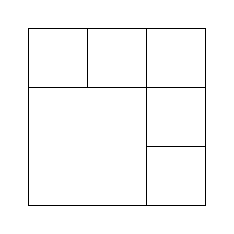
\begin{tikzpicture}[scale=.75]
    \draw (0,0) rectangle (3,3) (0,0) rectangle (2,2) (1,2) -- (1,3) (2,2) -- (2,3) (2,2) -- (3,2) (2,1)-- (3,1);
  \end{tikzpicture}
\end{center}
Prove, using strong induction, that it is possible to cut a square into $n$ smaller squares for any $n \ge 6$.  Hint: you will need three base cases.



\end{questions}
\end{document}
